% Options for packages loaded elsewhere
% Options for packages loaded elsewhere
\PassOptionsToPackage{unicode}{hyperref}
\PassOptionsToPackage{hyphens}{url}
\PassOptionsToPackage{dvipsnames,svgnames,x11names}{xcolor}
%
\documentclass[
  11pt,
  a4paper,
  DIV=11,
  numbers=noendperiod]{scrartcl}
\usepackage{xcolor}
\usepackage[lmargin=2cm,rmargin=2cm,tmargin=2cm,bmargin=2cm]{geometry}
\usepackage{amsmath,amssymb}
\setcounter{secnumdepth}{-\maxdimen} % remove section numbering
\usepackage{iftex}
\ifPDFTeX
  \usepackage[T1]{fontenc}
  \usepackage[utf8]{inputenc}
  \usepackage{textcomp} % provide euro and other symbols
\else % if luatex or xetex
  \usepackage{unicode-math} % this also loads fontspec
  \defaultfontfeatures{Scale=MatchLowercase}
  \defaultfontfeatures[\rmfamily]{Ligatures=TeX,Scale=1}
\fi
\usepackage{lmodern}
\ifPDFTeX\else
  % xetex/luatex font selection
\fi
% Use upquote if available, for straight quotes in verbatim environments
\IfFileExists{upquote.sty}{\usepackage{upquote}}{}
\IfFileExists{microtype.sty}{% use microtype if available
  \usepackage[]{microtype}
  \UseMicrotypeSet[protrusion]{basicmath} % disable protrusion for tt fonts
}{}
\makeatletter
\@ifundefined{KOMAClassName}{% if non-KOMA class
  \IfFileExists{parskip.sty}{%
    \usepackage{parskip}
  }{% else
    \setlength{\parindent}{0pt}
    \setlength{\parskip}{6pt plus 2pt minus 1pt}}
}{% if KOMA class
  \KOMAoptions{parskip=half}}
\makeatother
% Make \paragraph and \subparagraph free-standing
\makeatletter
\ifx\paragraph\undefined\else
  \let\oldparagraph\paragraph
  \renewcommand{\paragraph}{
    \@ifstar
      \xxxParagraphStar
      \xxxParagraphNoStar
  }
  \newcommand{\xxxParagraphStar}[1]{\oldparagraph*{#1}\mbox{}}
  \newcommand{\xxxParagraphNoStar}[1]{\oldparagraph{#1}\mbox{}}
\fi
\ifx\subparagraph\undefined\else
  \let\oldsubparagraph\subparagraph
  \renewcommand{\subparagraph}{
    \@ifstar
      \xxxSubParagraphStar
      \xxxSubParagraphNoStar
  }
  \newcommand{\xxxSubParagraphStar}[1]{\oldsubparagraph*{#1}\mbox{}}
  \newcommand{\xxxSubParagraphNoStar}[1]{\oldsubparagraph{#1}\mbox{}}
\fi
\makeatother

\usepackage{color}
\usepackage{fancyvrb}
\newcommand{\VerbBar}{|}
\newcommand{\VERB}{\Verb[commandchars=\\\{\}]}
\DefineVerbatimEnvironment{Highlighting}{Verbatim}{commandchars=\\\{\}}
% Add ',fontsize=\small' for more characters per line
\usepackage{framed}
\definecolor{shadecolor}{RGB}{241,243,245}
\newenvironment{Shaded}{\begin{snugshade}}{\end{snugshade}}
\newcommand{\AlertTok}[1]{\textcolor[rgb]{0.68,0.00,0.00}{#1}}
\newcommand{\AnnotationTok}[1]{\textcolor[rgb]{0.37,0.37,0.37}{#1}}
\newcommand{\AttributeTok}[1]{\textcolor[rgb]{0.40,0.45,0.13}{#1}}
\newcommand{\BaseNTok}[1]{\textcolor[rgb]{0.68,0.00,0.00}{#1}}
\newcommand{\BuiltInTok}[1]{\textcolor[rgb]{0.00,0.23,0.31}{#1}}
\newcommand{\CharTok}[1]{\textcolor[rgb]{0.13,0.47,0.30}{#1}}
\newcommand{\CommentTok}[1]{\textcolor[rgb]{0.37,0.37,0.37}{#1}}
\newcommand{\CommentVarTok}[1]{\textcolor[rgb]{0.37,0.37,0.37}{\textit{#1}}}
\newcommand{\ConstantTok}[1]{\textcolor[rgb]{0.56,0.35,0.01}{#1}}
\newcommand{\ControlFlowTok}[1]{\textcolor[rgb]{0.00,0.23,0.31}{\textbf{#1}}}
\newcommand{\DataTypeTok}[1]{\textcolor[rgb]{0.68,0.00,0.00}{#1}}
\newcommand{\DecValTok}[1]{\textcolor[rgb]{0.68,0.00,0.00}{#1}}
\newcommand{\DocumentationTok}[1]{\textcolor[rgb]{0.37,0.37,0.37}{\textit{#1}}}
\newcommand{\ErrorTok}[1]{\textcolor[rgb]{0.68,0.00,0.00}{#1}}
\newcommand{\ExtensionTok}[1]{\textcolor[rgb]{0.00,0.23,0.31}{#1}}
\newcommand{\FloatTok}[1]{\textcolor[rgb]{0.68,0.00,0.00}{#1}}
\newcommand{\FunctionTok}[1]{\textcolor[rgb]{0.28,0.35,0.67}{#1}}
\newcommand{\ImportTok}[1]{\textcolor[rgb]{0.00,0.46,0.62}{#1}}
\newcommand{\InformationTok}[1]{\textcolor[rgb]{0.37,0.37,0.37}{#1}}
\newcommand{\KeywordTok}[1]{\textcolor[rgb]{0.00,0.23,0.31}{\textbf{#1}}}
\newcommand{\NormalTok}[1]{\textcolor[rgb]{0.00,0.23,0.31}{#1}}
\newcommand{\OperatorTok}[1]{\textcolor[rgb]{0.37,0.37,0.37}{#1}}
\newcommand{\OtherTok}[1]{\textcolor[rgb]{0.00,0.23,0.31}{#1}}
\newcommand{\PreprocessorTok}[1]{\textcolor[rgb]{0.68,0.00,0.00}{#1}}
\newcommand{\RegionMarkerTok}[1]{\textcolor[rgb]{0.00,0.23,0.31}{#1}}
\newcommand{\SpecialCharTok}[1]{\textcolor[rgb]{0.37,0.37,0.37}{#1}}
\newcommand{\SpecialStringTok}[1]{\textcolor[rgb]{0.13,0.47,0.30}{#1}}
\newcommand{\StringTok}[1]{\textcolor[rgb]{0.13,0.47,0.30}{#1}}
\newcommand{\VariableTok}[1]{\textcolor[rgb]{0.07,0.07,0.07}{#1}}
\newcommand{\VerbatimStringTok}[1]{\textcolor[rgb]{0.13,0.47,0.30}{#1}}
\newcommand{\WarningTok}[1]{\textcolor[rgb]{0.37,0.37,0.37}{\textit{#1}}}

\usepackage{longtable,booktabs,array}
\usepackage{calc} % for calculating minipage widths
% Correct order of tables after \paragraph or \subparagraph
\usepackage{etoolbox}
\makeatletter
\patchcmd\longtable{\par}{\if@noskipsec\mbox{}\fi\par}{}{}
\makeatother
% Allow footnotes in longtable head/foot
\IfFileExists{footnotehyper.sty}{\usepackage{footnotehyper}}{\usepackage{footnote}}
\makesavenoteenv{longtable}
\usepackage{graphicx}
\makeatletter
\newsavebox\pandoc@box
\newcommand*\pandocbounded[1]{% scales image to fit in text height/width
  \sbox\pandoc@box{#1}%
  \Gscale@div\@tempa{\textheight}{\dimexpr\ht\pandoc@box+\dp\pandoc@box\relax}%
  \Gscale@div\@tempb{\linewidth}{\wd\pandoc@box}%
  \ifdim\@tempb\p@<\@tempa\p@\let\@tempa\@tempb\fi% select the smaller of both
  \ifdim\@tempa\p@<\p@\scalebox{\@tempa}{\usebox\pandoc@box}%
  \else\usebox{\pandoc@box}%
  \fi%
}
% Set default figure placement to htbp
\def\fps@figure{htbp}
\makeatother





\setlength{\emergencystretch}{3em} % prevent overfull lines

\providecommand{\tightlist}{%
  \setlength{\itemsep}{0pt}\setlength{\parskip}{0pt}}



 


\KOMAoption{captions}{tableheading}
\makeatletter
\@ifpackageloaded{caption}{}{\usepackage{caption}}
\AtBeginDocument{%
\ifdefined\contentsname
  \renewcommand*\contentsname{Table of contents}
\else
  \newcommand\contentsname{Table of contents}
\fi
\ifdefined\listfigurename
  \renewcommand*\listfigurename{List of Figures}
\else
  \newcommand\listfigurename{List of Figures}
\fi
\ifdefined\listtablename
  \renewcommand*\listtablename{List of Tables}
\else
  \newcommand\listtablename{List of Tables}
\fi
\ifdefined\figurename
  \renewcommand*\figurename{Figure}
\else
  \newcommand\figurename{Figure}
\fi
\ifdefined\tablename
  \renewcommand*\tablename{Table}
\else
  \newcommand\tablename{Table}
\fi
}
\@ifpackageloaded{float}{}{\usepackage{float}}
\floatstyle{ruled}
\@ifundefined{c@chapter}{\newfloat{codelisting}{h}{lop}}{\newfloat{codelisting}{h}{lop}[chapter]}
\floatname{codelisting}{Listing}
\newcommand*\listoflistings{\listof{codelisting}{List of Listings}}
\makeatother
\makeatletter
\makeatother
\makeatletter
\@ifpackageloaded{caption}{}{\usepackage{caption}}
\@ifpackageloaded{subcaption}{}{\usepackage{subcaption}}
\makeatother
\usepackage{bookmark}
\IfFileExists{xurl.sty}{\usepackage{xurl}}{} % add URL line breaks if available
\urlstyle{same}
\hypersetup{
  pdftitle={Migration Dynamics and Quality of Life Index},
  colorlinks=true,
  linkcolor={blue},
  filecolor={Maroon},
  citecolor={Blue},
  urlcolor={Blue},
  pdfcreator={LaTeX via pandoc}}


\title{Migration Dynamics and Quality of Life Index}
\author{}
\date{}
\begin{document}
\maketitle


Welcome to our project page.

\emph{Team BU-R-SEL}

\href{https://emu-hacettepe-analytics.github.io/emu660-spring2026-Selindznn/project.html}{Selin
DÜZEN}

\href{https://emu-hacettepe-analytics.github.io/emu660-spring2026-burcubaris/project.html}{Burcu
BARIŞ}

\section{1. Project Overview and
Scope}\label{project-overview-and-scope}

Migration is not merely the geographical displacement of individuals; it
is also a reflection of economic pursuits, social opportunities, and
structural quality in a region. In Turkey, the difference in development
and living standards between provinces constitutes one of the primary
dynamics of internal migration movements.

In this project, using TUIK (Turkish Statistical Institute) data, we aim
to examine the multidimensional relationship between Net Migration (Net
Migration = Migrant Receiving - Migrant Giving) figures for all 81
provinces of Turkiye and the Livability Index indicators in these
provinces using analytical methods. Our goal is to reveal, through data
analytics and statistical models, which vital factors (economy,
education, health, environmental quality, security, etc.) cause people
to leave their current cities or move to specific cities.

\emph{Creating Migration Profiles:} To identify the ``Net Migration
Champions'' (provinces receiving the most net migrants) and ``Migration
Sources'' (provinces giving the most net migrants) in Turkiye and to map
them geographically.

\emph{The Impact of Livability Dimensions:} To statistically demonstrate
which of the sub-components of the livability index (Income and Wealth,
Health, Education, Environment, Security, etc.) are more dominant
``push'' or ``pull'' forces influencing migration decisions.

\section{2. Data}\label{data}

\subsection{2.1 Data Source}\label{data-source}

The datasets used in the project are:

1.\href{https://veriportali.tuik.gov.tr/api/tr/data/downloads?t=i&p=btt\%2FI0Npd\%2BLvtOvCSZRIUZxbvXE3lIAf5bE6X3CdLQJxPknvezk\%2BE6i3Md3GTPYHYMhzGdG2vbYkzOXomic6rY8F\%2FyL8NGud1ChYCxoEgy5FkIT\%2BMezMLoMVyKJUHwSgAQ\%2BDeuZaUgEdXmyanOwSEQ\%3D\%3D}{Population
size of the provinces}

2.\href{https://veriportali.tuik.gov.tr/api/tr/data/downloads?t=i&p=\%2FMyiBh3DmS\%2Bv\%2BBjCf9\%2BzPq\%2B96lw8HZTF50uTl9jqBks\%2BK5WE6sQNt\%2Fqka0J5\%2BImWGTGxKxiPcrz7kNG6I3rKkrLi\%2B8mZkMkz9reke8\%2BHd\%2Fo\%3D}{Migration
received by provinces according to the reason for migration}

3.\href{https://veriportali.tuik.gov.tr/api/tr/data/downloads?t=i&p=\%2FMyiBh3DmS\%2Bv\%2BBjCf9\%2BzPq\%2B96lw8HZTF50uTl9jqBks\%2BK5WE6sQNt\%2Fqka0J5\%2BImWGTGxKxiPcrz7kNG6I3rKkrLi\%2B8mZkMkz9reke8\%2BHd\%2Fo\%3D}{Migration
rates by provinces according to the reason for migration}

4.{[}Net migration rate for provinces according to reasons for
migration{]} Calculated as ``Migration Outgoing - Migration Incoming''

3.\href{https://veriportali.tuik.gov.tr/api/tr/data/downloads?t=i&p=5IS1p1Z\%2Btvlc0qxFhZzbC9g6NOWXugwdILs8mAMegx5w5sIpUqxydG6\%2B5\%2FWn1HGIIXJVqd\%2Fwn\%2B78duD2fsK84VEREA5Sn4QY5oeOWRHZRvVYOaDudiOCwll9hFpmp5W}{Life
Index Rankings and Index Values by Province}

\subsection{2.2 General Information About
Data}\label{general-information-about-data}

Our dataset tracks migration metrics across all 81 provinces of
TC\textless rkiye from 2018 to 2024. It combines raw inbound/outbound
migration figures with detailed columns explaining 12 different reasons
for migration, cross-references them with the Turkish Statistical
Institute's (TCD0K) comprehensive Life Index scores, and shows the
relationships between them.

\subsection{2.3 Reason of Choice}\label{reason-of-choice}

We chose this data because migration cannot be explained solely by
economic factors. By combining net migration metrics with the
multidimensional Life Index (which assesses health, education, security,
and environment), we can reveal the relationship between internal
migration in TC\textless rkiye and life indices.

\subsection{2.4 Preprocessing}\label{preprocessing}

The net migration values are calculated using migration data received
and given by provinces in different Excel spreadsheets and the char
formatted values containing spaces in the data were updated to numeric
values.

\begin{Shaded}
\begin{Highlighting}[]
\CommentTok{\#install.packages("ggplot2") }
\CommentTok{\#install.packages("dplyr")   }
\CommentTok{\#install.packages("openxlsx")}
\CommentTok{\#install.packages("readxl")}

\CommentTok{\# 1. R\textquotesingle{}ın geçici işlemler için C diskinin altında temiz bir klasör kullanmasını sağlıyoruz}
\FunctionTok{write}\NormalTok{(}\StringTok{"TMPDIR = C:}\SpecialCharTok{\textbackslash{}\textbackslash{}}\StringTok{"}\NormalTok{, }\AttributeTok{file =} \FunctionTok{file.path}\NormalTok{(}\FunctionTok{Sys.getenv}\NormalTok{(}\StringTok{"HOME"}\NormalTok{), }\StringTok{".Renviron"}\NormalTok{), }\AttributeTok{append =} \ConstantTok{TRUE}\NormalTok{)}

\CommentTok{\# 2. Şimdi paketi tekrar yüklemeyi dene}
\CommentTok{\#install.packages("writexl")}

\CommentTok{\#install.packages("ggrepel")}
\FunctionTok{library}\NormalTok{(ggplot2)}
\FunctionTok{library}\NormalTok{(dplyr)}
\FunctionTok{library}\NormalTok{(readxl) }
\FunctionTok{library}\NormalTok{(writexl) }
\FunctionTok{library}\NormalTok{(stringr)}
\FunctionTok{library}\NormalTok{(forcats)}
\FunctionTok{library}\NormalTok{(tidyr)}
\FunctionTok{library}\NormalTok{(openxlsx)}
\FunctionTok{library}\NormalTok{(ggplot2)}
\FunctionTok{library}\NormalTok{(readxl)}
\FunctionTok{library}\NormalTok{(dplyr)}
\FunctionTok{library}\NormalTok{(ggrepel)}
\end{Highlighting}
\end{Shaded}

\subsubsection{2.4.1. Calculating net migration values and creating a
separate Excel file and checking and correcting numerical
values.}\label{calculating-net-migration-values-and-creating-a-separate-excel-file-and-checking-and-correcting-numerical-values.}

\begin{Shaded}
\begin{Highlighting}[]
\NormalTok{VerilenGoc }\OtherTok{\textless{}{-}} \FunctionTok{read\_excel}\NormalTok{(}\StringTok{"C:/emu660{-}spring2026{-}burcubaris/VerilenGoc.xlsx"}\NormalTok{, }\AttributeTok{col\_names =} \ConstantTok{TRUE}\NormalTok{)}
\NormalTok{AlinanGoc  }\OtherTok{\textless{}{-}} \FunctionTok{read\_excel}\NormalTok{(}\StringTok{"C:/emu660{-}spring2026{-}burcubaris/AlinanGoc.xlsx"}\NormalTok{, }\AttributeTok{col\_names =} \ConstantTok{TRUE}\NormalTok{)}
\NormalTok{toplam\_sutun }\OtherTok{\textless{}{-}} \FunctionTok{ncol}\NormalTok{(VerilenGoc)}
\NormalTok{fark\_df }\OtherTok{\textless{}{-}}\NormalTok{ VerilenGoc }
\ControlFlowTok{for}\NormalTok{ (i }\ControlFlowTok{in} \DecValTok{3}\SpecialCharTok{:}\NormalTok{toplam\_sutun) \{}
\NormalTok{  v\_clean }\OtherTok{\textless{}{-}} \FunctionTok{as.character}\NormalTok{(VerilenGoc[[i]])}
\NormalTok{  v\_clean }\OtherTok{\textless{}{-}} \FunctionTok{str\_replace\_all}\NormalTok{(v\_clean, }\StringTok{"}\SpecialCharTok{\textbackslash{}\textbackslash{}}\StringTok{s"}\NormalTok{, }\StringTok{""}\NormalTok{) }
\NormalTok{  VerilenGoc[[i]] }\OtherTok{\textless{}{-}} \FunctionTok{as.numeric}\NormalTok{(v\_clean)        }
\NormalTok{  a\_clean }\OtherTok{\textless{}{-}} \FunctionTok{as.character}\NormalTok{(AlinanGoc[[i]])}
\NormalTok{  a\_clean }\OtherTok{\textless{}{-}} \FunctionTok{str\_replace\_all}\NormalTok{(a\_clean, }\StringTok{"}\SpecialCharTok{\textbackslash{}\textbackslash{}}\StringTok{s"}\NormalTok{, }\StringTok{""}\NormalTok{)    }
\NormalTok{  AlinanGoc[[i]] }\OtherTok{\textless{}{-}} \FunctionTok{as.numeric}\NormalTok{(a\_clean)}
\NormalTok{\}}
\NormalTok{fark\_df[, }\DecValTok{3}\SpecialCharTok{:}\NormalTok{toplam\_sutun] }\OtherTok{\textless{}{-}}\NormalTok{ VerilenGoc[, }\DecValTok{3}\SpecialCharTok{:}\NormalTok{toplam\_sutun] }\SpecialCharTok{{-}}\NormalTok{ AlinanGoc[, }\DecValTok{3}\SpecialCharTok{:}\NormalTok{toplam\_sutun]}
\ControlFlowTok{for}\NormalTok{ (i }\ControlFlowTok{in} \DecValTok{3}\SpecialCharTok{:}\NormalTok{toplam\_sutun) \{}
\NormalTok{  fark\_df[[i]] }\OtherTok{\textless{}{-}} \FunctionTok{as.numeric}\NormalTok{(fark\_df[[i]])}
\NormalTok{\}}
\FunctionTok{write\_xlsx}\NormalTok{(fark\_df, }\StringTok{"C:/emu660{-}spring2026{-}burcubaris/NetGoc.xlsx"}\NormalTok{)}
\FunctionTok{print}\NormalTok{(VerilenGoc[, }\DecValTok{3}\SpecialCharTok{:}\NormalTok{toplam\_sutun])}
\end{Highlighting}
\end{Shaded}

\begin{verbatim}
# A tibble: 574 x 13
   `Toplam\r\nTotal` Tayin / iş değişikliği\r\nAssignat~1 İşe başlamak /\r\n i~2
               <dbl>                                <dbl>                  <dbl>
 1           2682673                               280980                 221022
 2             56108                                 5251                   4260
 3             21158                                 2069                   1663
 4             25035                                 2770                   2657
 5             30970                                 4427                   2483
 6             14446                                 1594                   1444
 7            150373                                18554                  11161
 8             71999                                 5522                   5242
 9             10400                                 1046                   1110
10             35832                                 2971                   3561
# i 564 more rows
# i abbreviated names:
#   1: `Tayin / iş değişikliği\r\nAssignation /\r\n change of job`,
#   2: `İşe başlamak /\r\n iş bulmak\r\nStarting / finding a job`
# i 10 more variables: `Eğitim\r\nEducation` <dbl>,
#   `Medeni durum değişikliği / ailevi nedenler\r\nChange of marital status / family\r\nrelated reasons` <dbl>,
#   `Daha iyi konut ve yaşam koşulları\r\n Better housing and living conditions` <dbl>, ...
\end{verbatim}

\subsubsection{2.4.2. Calculating net migration rate using population
data of provinces and creating an Excel
file.}\label{calculating-net-migration-rate-using-population-data-of-provinces-and-creating-an-excel-file.}

\begin{Shaded}
\begin{Highlighting}[]
\NormalTok{kaynak\_yolu }\OtherTok{\textless{}{-}} \StringTok{"C:/Users/Public/Documents/my\_repository\_emu660/emu660{-}spring2026{-}burcubaris/NetGoc.xlsx"}
\NormalTok{hedef\_yolu  }\OtherTok{\textless{}{-}} \StringTok{"C:/Users/Public/Documents/my\_repository\_emu660/emu660{-}spring2026{-}burcubaris/IlNufuslarii.xlsx"}

\NormalTok{df\_kaynak }\OtherTok{\textless{}{-}} \FunctionTok{read\_excel}\NormalTok{(kaynak\_yolu, }\AttributeTok{col\_names =} \ConstantTok{TRUE}\NormalTok{)}

\NormalTok{NetGocVerisi }\OtherTok{\textless{}{-}}\NormalTok{ df\_kaynak[}\DecValTok{1}\SpecialCharTok{:}\DecValTok{82}\NormalTok{, }\DecValTok{3}\NormalTok{, drop }\OtherTok{=} \ConstantTok{TRUE}\NormalTok{] }
\NormalTok{wb }\OtherTok{\textless{}{-}} \FunctionTok{loadWorkbook}\NormalTok{(hedef\_yolu)}
\FunctionTok{writeData}\NormalTok{(wb, }\AttributeTok{sheet =} \DecValTok{1}\NormalTok{, }\AttributeTok{x =} \StringTok{"Net GC6C\textquotesingle{}"}\NormalTok{, }\AttributeTok{startCol =} \DecValTok{3}\NormalTok{, }\AttributeTok{startRow =} \DecValTok{1}\NormalTok{, }\AttributeTok{colNames =} \ConstantTok{FALSE}\NormalTok{)}
\FunctionTok{writeData}\NormalTok{(wb, }\AttributeTok{sheet =} \DecValTok{1}\NormalTok{, }\AttributeTok{x =}\NormalTok{ NetGocVerisi, }\AttributeTok{startCol =} \DecValTok{3}\NormalTok{, }\AttributeTok{startRow =} \DecValTok{2}\NormalTok{, }\AttributeTok{colNames =} \ConstantTok{FALSE}\NormalTok{)}

\FunctionTok{saveWorkbook}\NormalTok{(wb, hedef\_yolu, }\AttributeTok{overwrite =} \ConstantTok{TRUE}\NormalTok{)}
\end{Highlighting}
\end{Shaded}

\section{3. Analysis}\label{analysis}

\subsection{3.1 Exploratory Data
Analysis}\label{exploratory-data-analysis}

\subsubsection{3.1.1. Changes in Total Migration Values by Year
(2018-2024)}\label{changes-in-total-migration-values-by-year-2018-2024}

The changes in the total amount of migration over the years were shown
graphically.

\begin{Shaded}
\begin{Highlighting}[]
\NormalTok{grafik\_verisi }\OtherTok{\textless{}{-}}\NormalTok{ VerilenGoc[VerilenGoc[, }\DecValTok{2}\NormalTok{] }\SpecialCharTok{==} \StringTok{"Toplam{-}Total"}\NormalTok{, ]}
\FunctionTok{print}\NormalTok{(grafik\_verisi)}
\end{Highlighting}
\end{Shaded}

\begin{verbatim}
# A tibble: 7 x 15
  `Yıl\r\nYear` `İl\r\nProvince` `Toplam\r\nTotal` Tayin / iş değişikliği\r\nA~1
          <dbl> <chr>                        <dbl>                         <dbl>
1          2024 Toplam-Total               2682673                        280980
2          2023 Toplam-Total               3450953                        320142
3          2022 Toplam-Total               2791156                        301335
4          2021 Toplam-Total               2777797                        265537
5          2020 Toplam-Total               2258726                        257027
6          2019 Toplam-Total               2806123                        262833
7          2018 Toplam-Total               3057606                        315849
# i abbreviated name:
#   1: `Tayin / iş değişikliği\r\nAssignation /\r\n change of job`
# i 11 more variables:
#   `İşe başlamak /\r\n iş bulmak\r\nStarting / finding a job` <dbl>,
#   `Eğitim\r\nEducation` <dbl>,
#   `Medeni durum değişikliği / ailevi nedenler\r\nChange of marital status / family\r\nrelated reasons` <dbl>,
#   `Daha iyi konut ve yaşam koşulları\r\n Better housing and living conditions` <dbl>, ...
\end{verbatim}

\begin{Shaded}
\begin{Highlighting}[]
\FunctionTok{head}\NormalTok{(grafik\_verisi)}
\end{Highlighting}
\end{Shaded}

\begin{verbatim}
# A tibble: 6 x 15
  `Yıl\r\nYear` `İl\r\nProvince` `Toplam\r\nTotal` Tayin / iş değişikliği\r\nA~1
          <dbl> <chr>                        <dbl>                         <dbl>
1          2024 Toplam-Total               2682673                        280980
2          2023 Toplam-Total               3450953                        320142
3          2022 Toplam-Total               2791156                        301335
4          2021 Toplam-Total               2777797                        265537
5          2020 Toplam-Total               2258726                        257027
6          2019 Toplam-Total               2806123                        262833
# i abbreviated name:
#   1: `Tayin / iş değişikliği\r\nAssignation /\r\n change of job`
# i 11 more variables:
#   `İşe başlamak /\r\n iş bulmak\r\nStarting / finding a job` <dbl>,
#   `Eğitim\r\nEducation` <dbl>,
#   `Medeni durum değişikliği / ailevi nedenler\r\nChange of marital status / family\r\nrelated reasons` <dbl>,
#   `Daha iyi konut ve yaşam koşulları\r\n Better housing and living conditions` <dbl>, ...
\end{verbatim}

\begin{Shaded}
\begin{Highlighting}[]
\NormalTok{yil }\OtherTok{\textless{}{-}} \FunctionTok{factor}\NormalTok{(grafik\_verisi[[}\DecValTok{1}\NormalTok{]], }\AttributeTok{levels =} \FunctionTok{sort}\NormalTok{(}\FunctionTok{unique}\NormalTok{(grafik\_verisi[[}\DecValTok{1}\NormalTok{]]), }\AttributeTok{decreasing =} \ConstantTok{TRUE}\NormalTok{))}
\NormalTok{goc\_miktari  }\OtherTok{\textless{}{-}} \FunctionTok{as.numeric}\NormalTok{(grafik\_verisi[[}\DecValTok{3}\NormalTok{]])}\SpecialCharTok{/}\DecValTok{1000}  

\FunctionTok{ggplot}\NormalTok{(}\AttributeTok{data =}\NormalTok{ grafik\_verisi, }\FunctionTok{aes}\NormalTok{(}\AttributeTok{x =}\NormalTok{ yil, }\AttributeTok{y =}\NormalTok{ goc\_miktari)) }\SpecialCharTok{+}
  \FunctionTok{geom\_col}\NormalTok{(}\AttributeTok{fill =} \StringTok{"steelblue"}\NormalTok{, }\AttributeTok{alpha =} \FloatTok{0.7}\NormalTok{) }\SpecialCharTok{+} 
  \FunctionTok{geom\_line}\NormalTok{(}\AttributeTok{color =} \StringTok{"black"}\NormalTok{, }\AttributeTok{size =} \DecValTok{2}\NormalTok{) }\SpecialCharTok{+} 
  \FunctionTok{geom\_point}\NormalTok{(}\AttributeTok{color =} \StringTok{"darkred"}\NormalTok{, }\AttributeTok{size =} \DecValTok{3}\NormalTok{) }\SpecialCharTok{+}
  \FunctionTok{geom\_text}\NormalTok{(}\FunctionTok{aes}\NormalTok{(}\AttributeTok{label =} \FunctionTok{round}\NormalTok{(goc\_miktari, }\DecValTok{1}\NormalTok{)), }\AttributeTok{vjust =} \SpecialCharTok{{-}}\FloatTok{0.5}\NormalTok{, }\AttributeTok{size =} \FloatTok{3.5}\NormalTok{) }\SpecialCharTok{+}
  \FunctionTok{labs}\NormalTok{(}
    \AttributeTok{title =} \StringTok{"YD1llara GC6re Toplam Verilen GC6C\textquotesingle{} MiktarD1"}\NormalTok{,}
    \AttributeTok{x =} \StringTok{"YD1l"}\NormalTok{,}
    \AttributeTok{y =} \StringTok{"GC6C\textquotesingle{} MiktarD1 (x1.000)"}
\NormalTok{  )}
\end{Highlighting}
\end{Shaded}

\pandocbounded{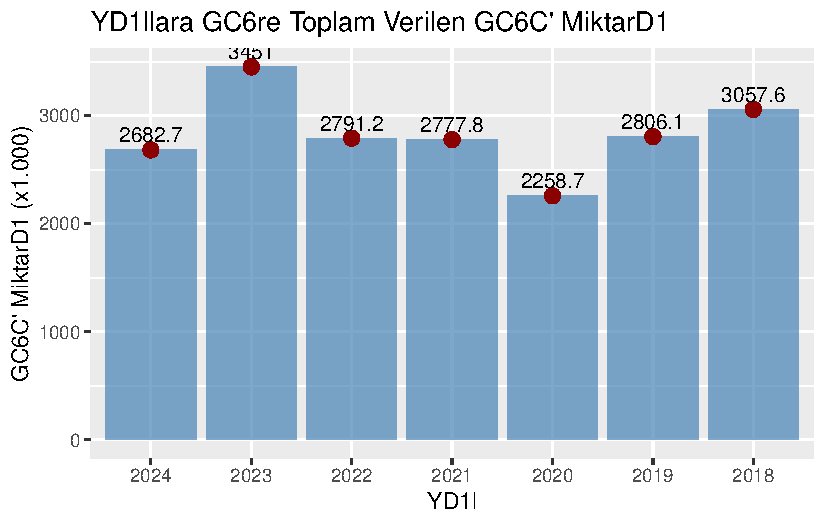
\includegraphics[keepaspectratio]{project_files/figure-pdf/unnamed-chunk-4-1.pdf}}

\subsubsection{3.1.2. Changes in Total Migration Values by Year for
Ankara
Provience}\label{changes-in-total-migration-values-by-year-for-ankara-provience}

The graphic shows the changes in total migration amounts over the years
for Ankara province.

\begin{Shaded}
\begin{Highlighting}[]
\NormalTok{grafik\_verisi }\OtherTok{\textless{}{-}}\NormalTok{ VerilenGoc[VerilenGoc[, }\DecValTok{2}\NormalTok{] }\SpecialCharTok{==} \StringTok{"Ankara"}\NormalTok{, ]}
\FunctionTok{print}\NormalTok{(grafik\_verisi)}
\end{Highlighting}
\end{Shaded}

\begin{verbatim}
# A tibble: 7 x 15
  `Yıl\r\nYear` `İl\r\nProvince` `Toplam\r\nTotal` Tayin / iş değişikliği\r\nA~1
          <dbl> <chr>                        <dbl>                         <dbl>
1          2024 Ankara                      150373                         18554
2          2023 Ankara                      208740                         21809
3          2022 Ankara                      161912                         18930
4          2021 Ankara                      165604                         19685
5          2020 Ankara                      141165                         19852
6          2019 Ankara                      154464                         18398
7          2018 Ankara                      221747                         24631
# i abbreviated name:
#   1: `Tayin / iş değişikliği\r\nAssignation /\r\n change of job`
# i 11 more variables:
#   `İşe başlamak /\r\n iş bulmak\r\nStarting / finding a job` <dbl>,
#   `Eğitim\r\nEducation` <dbl>,
#   `Medeni durum değişikliği / ailevi nedenler\r\nChange of marital status / family\r\nrelated reasons` <dbl>,
#   `Daha iyi konut ve yaşam koşulları\r\n Better housing and living conditions` <dbl>, ...
\end{verbatim}

\begin{Shaded}
\begin{Highlighting}[]
\FunctionTok{head}\NormalTok{(grafik\_verisi)}
\end{Highlighting}
\end{Shaded}

\begin{verbatim}
# A tibble: 6 x 15
  `Yıl\r\nYear` `İl\r\nProvince` `Toplam\r\nTotal` Tayin / iş değişikliği\r\nA~1
          <dbl> <chr>                        <dbl>                         <dbl>
1          2024 Ankara                      150373                         18554
2          2023 Ankara                      208740                         21809
3          2022 Ankara                      161912                         18930
4          2021 Ankara                      165604                         19685
5          2020 Ankara                      141165                         19852
6          2019 Ankara                      154464                         18398
# i abbreviated name:
#   1: `Tayin / iş değişikliği\r\nAssignation /\r\n change of job`
# i 11 more variables:
#   `İşe başlamak /\r\n iş bulmak\r\nStarting / finding a job` <dbl>,
#   `Eğitim\r\nEducation` <dbl>,
#   `Medeni durum değişikliği / ailevi nedenler\r\nChange of marital status / family\r\nrelated reasons` <dbl>,
#   `Daha iyi konut ve yaşam koşulları\r\n Better housing and living conditions` <dbl>, ...
\end{verbatim}

\begin{Shaded}
\begin{Highlighting}[]
\NormalTok{yil }\OtherTok{\textless{}{-}} \FunctionTok{factor}\NormalTok{(grafik\_verisi[[}\DecValTok{1}\NormalTok{]], }\AttributeTok{levels =} \FunctionTok{sort}\NormalTok{(}\FunctionTok{unique}\NormalTok{(grafik\_verisi[[}\DecValTok{1}\NormalTok{]]), }\AttributeTok{decreasing =} \ConstantTok{TRUE}\NormalTok{))}
\NormalTok{goc\_miktari  }\OtherTok{\textless{}{-}} \FunctionTok{as.numeric}\NormalTok{(grafik\_verisi[[}\DecValTok{3}\NormalTok{]])}\SpecialCharTok{/}\DecValTok{1000}  

\FunctionTok{ggplot}\NormalTok{(}\AttributeTok{data =}\NormalTok{ grafik\_verisi, }\FunctionTok{aes}\NormalTok{(}\AttributeTok{x =}\NormalTok{ yil, }\AttributeTok{y =}\NormalTok{ goc\_miktari)) }\SpecialCharTok{+}
  \FunctionTok{geom\_col}\NormalTok{(}\AttributeTok{fill =} \StringTok{"steelblue"}\NormalTok{, }\AttributeTok{alpha =} \FloatTok{0.7}\NormalTok{) }\SpecialCharTok{+} 
  \FunctionTok{geom\_line}\NormalTok{(}\AttributeTok{color =} \StringTok{"black"}\NormalTok{, }\AttributeTok{size =} \DecValTok{2}\NormalTok{) }\SpecialCharTok{+} 
  \FunctionTok{geom\_point}\NormalTok{(}\AttributeTok{color =} \StringTok{"darkred"}\NormalTok{, }\AttributeTok{size =} \DecValTok{3}\NormalTok{) }\SpecialCharTok{+}
  \FunctionTok{geom\_text}\NormalTok{(}\FunctionTok{aes}\NormalTok{(}\AttributeTok{label =} \FunctionTok{round}\NormalTok{(goc\_miktari, }\DecValTok{1}\NormalTok{)), }\AttributeTok{vjust =} \SpecialCharTok{{-}}\FloatTok{0.5}\NormalTok{, }\AttributeTok{size =} \FloatTok{3.5}\NormalTok{) }\SpecialCharTok{+}
  \FunctionTok{labs}\NormalTok{(}
    \AttributeTok{title =} \StringTok{"Ankara iC\textquotesingle{}in YD1llara GC6re Toplam Verilen GC6C\textquotesingle{} MiktarD1"}\NormalTok{,}
    \AttributeTok{x =} \StringTok{"YD1l"}\NormalTok{,}
    \AttributeTok{y =} \StringTok{"GC6C\textquotesingle{} MiktarD1 (x1.000)"}
\NormalTok{  )}
\end{Highlighting}
\end{Shaded}

\pandocbounded{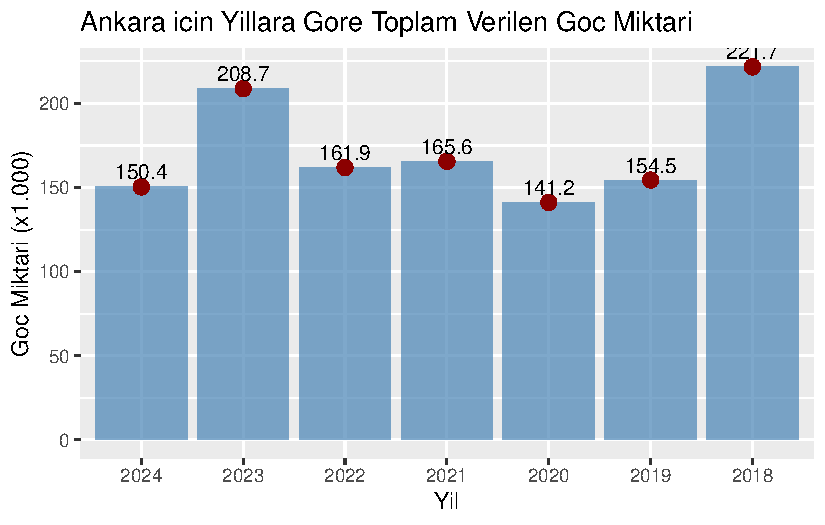
\includegraphics[keepaspectratio]{project_files/figure-pdf/unnamed-chunk-5-1.pdf}}

\subsubsection{3.1.3. Migration Figures by Province in
2024}\label{migration-figures-by-province-in-2024}

\begin{Shaded}
\begin{Highlighting}[]
\NormalTok{AlinanGoc  }\OtherTok{\textless{}{-}} \FunctionTok{read\_excel}\NormalTok{(}\StringTok{"C:/Users/Public/Documents/my\_repository\_emu660/emu660{-}spring2026{-}burcubaris/AlinanGoc.xlsx"}\NormalTok{,}\AttributeTok{col\_names =} \ConstantTok{TRUE}\NormalTok{)}

\FunctionTok{colnames}\NormalTok{(AlinanGoc)[}\DecValTok{1}\SpecialCharTok{:}\DecValTok{3}\NormalTok{] }\OtherTok{\textless{}{-}} \FunctionTok{c}\NormalTok{(}\StringTok{"Yil"}\NormalTok{, }\StringTok{"Il"}\NormalTok{, }\StringTok{"Goc\_Miktari"}\NormalTok{)}
\NormalTok{veri\_2024 }\OtherTok{\textless{}{-}} \FunctionTok{subset}\NormalTok{(AlinanGoc, Yil }\SpecialCharTok{==} \DecValTok{2024} \SpecialCharTok{\&}\NormalTok{ Il }\SpecialCharTok{!=} \StringTok{"Toplam{-}Total"}\NormalTok{)}
\NormalTok{veri\_2024}\SpecialCharTok{$}\NormalTok{Goc\_Miktari\_Bin }\OtherTok{\textless{}{-}}\NormalTok{ veri\_2024}\SpecialCharTok{$}\NormalTok{Goc\_Miktari }\SpecialCharTok{/} \DecValTok{1000}


\FunctionTok{ggplot}\NormalTok{(veri\_2024, }\FunctionTok{aes}\NormalTok{(}\AttributeTok{x =}\NormalTok{ Goc\_Miktari\_Bin, }\AttributeTok{y =} \FunctionTok{reorder}\NormalTok{(Il, Goc\_Miktari\_Bin))) }\SpecialCharTok{+}
  \FunctionTok{geom\_col}\NormalTok{(}\FunctionTok{aes}\NormalTok{(}\AttributeTok{fill =}\NormalTok{ Goc\_Miktari\_Bin }\SpecialCharTok{\textgreater{}} \DecValTok{0}\NormalTok{)) }\SpecialCharTok{+}
  \FunctionTok{scale\_fill\_manual}\NormalTok{(}\AttributeTok{values =} \FunctionTok{c}\NormalTok{(}\StringTok{"coral"}\NormalTok{, }\StringTok{"skyblue"}\NormalTok{), }\AttributeTok{guide =} \StringTok{"none"}\NormalTok{) }\SpecialCharTok{+}
  \FunctionTok{theme\_minimal}\NormalTok{() }\SpecialCharTok{+}
  \FunctionTok{labs}\NormalTok{(}
    \AttributeTok{title =} \StringTok{"2024 YD1lD1 D0llerin AlD1nan GC6C\textquotesingle{} MiktarlarD1"}\NormalTok{,}
    \AttributeTok{x =} \StringTok{"AlD1nan GC6C\textquotesingle{} MiktarD1 (Bin KiEi)"}\NormalTok{,}
    \AttributeTok{y =} \StringTok{"D0ller"}
\NormalTok{  )}
\end{Highlighting}
\end{Shaded}

\pandocbounded{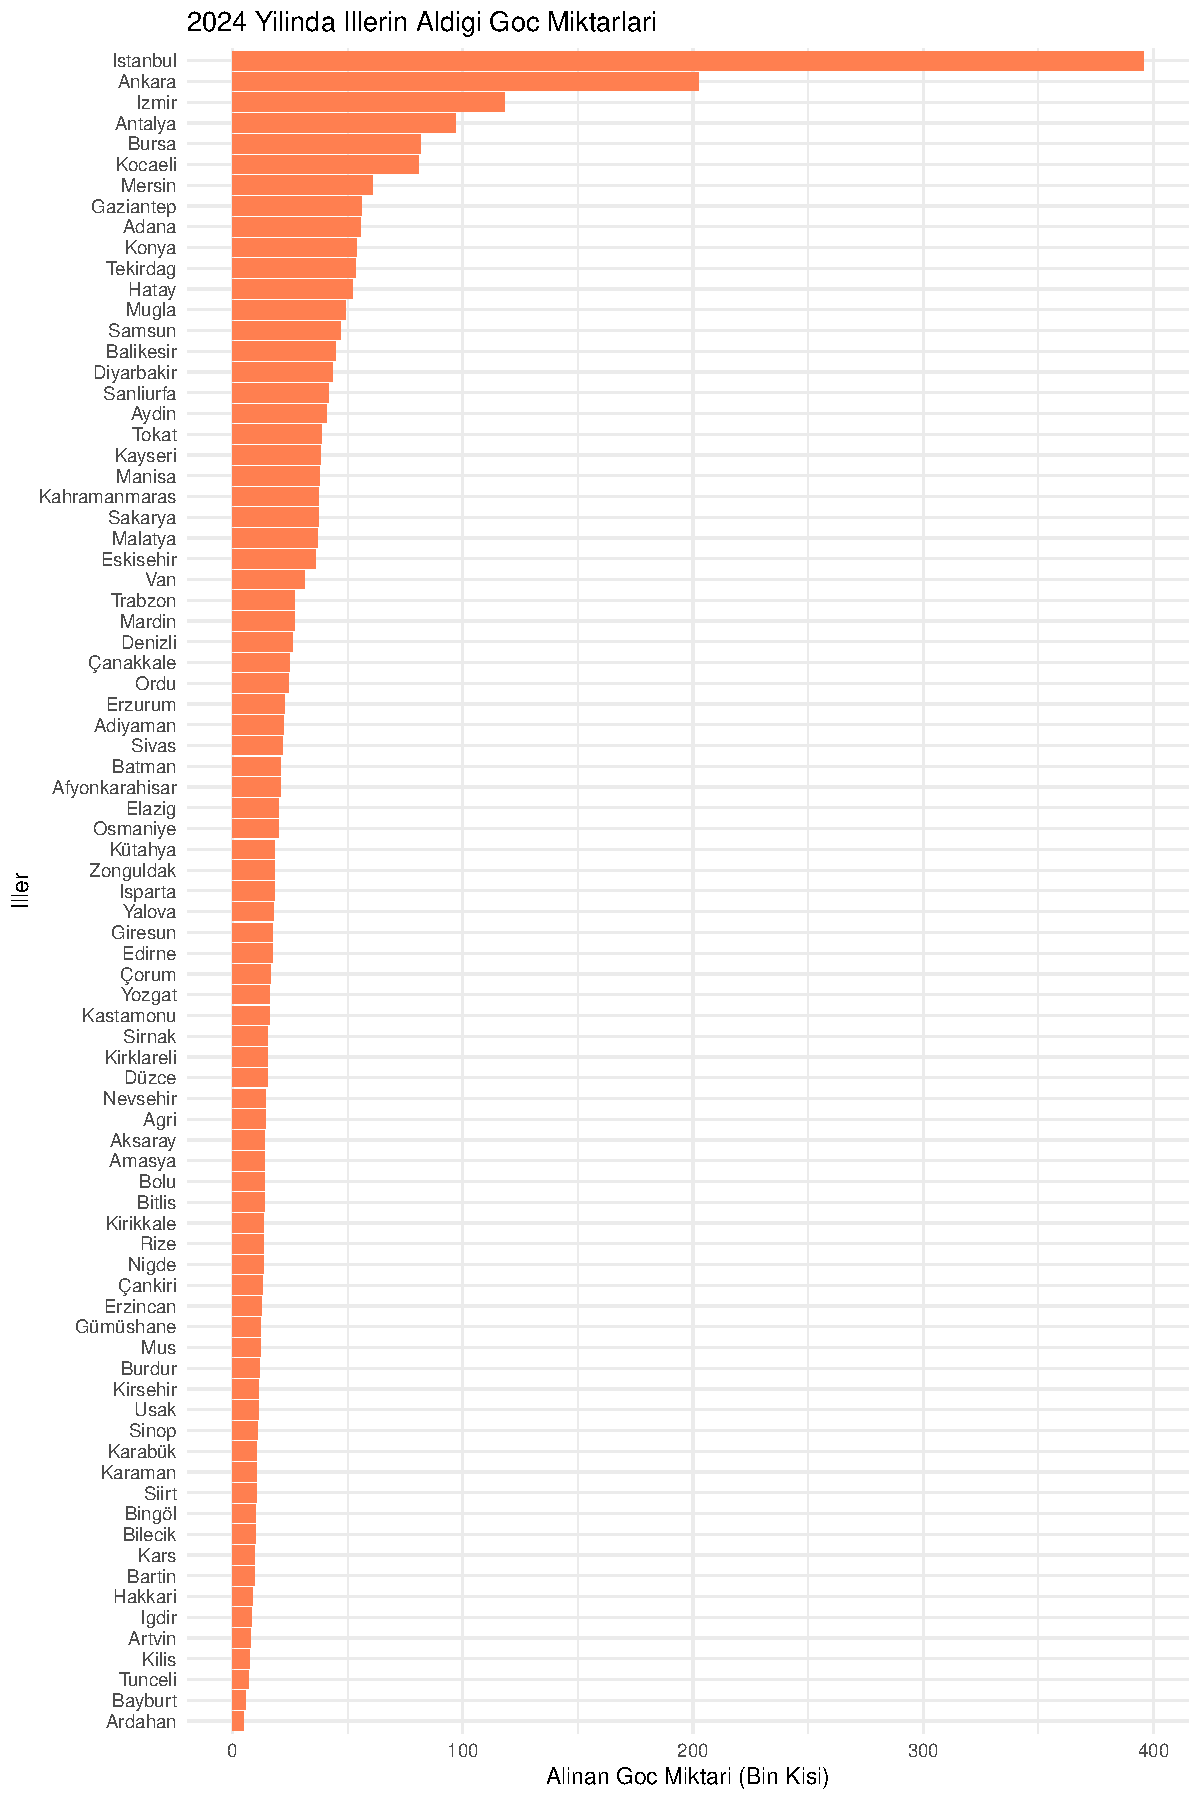
\includegraphics[keepaspectratio]{project_files/figure-pdf/unnamed-chunk-6-1.pdf}}

\subsubsection{3.1.4. Net Migration Figures of Provinces in
2024}\label{net-migration-figures-of-provinces-in-2024}

A graphical representation of the calculation made using the previously
calculated data given migration-received migration data.

\begin{Shaded}
\begin{Highlighting}[]
\NormalTok{NetGoc  }\OtherTok{\textless{}{-}} \FunctionTok{read\_excel}\NormalTok{(}\StringTok{"C:/Users/Public/Documents/my\_repository\_emu660/emu660{-}spring2026{-}burcubaris/NetGoc.xlsx"}\NormalTok{,}\AttributeTok{col\_names =} \ConstantTok{TRUE}\NormalTok{)}

\FunctionTok{colnames}\NormalTok{(NetGoc)[}\DecValTok{1}\SpecialCharTok{:}\DecValTok{3}\NormalTok{] }\OtherTok{\textless{}{-}} \FunctionTok{c}\NormalTok{(}\StringTok{"Yil"}\NormalTok{, }\StringTok{"Il"}\NormalTok{, }\StringTok{"Goc\_Miktari"}\NormalTok{)}
\NormalTok{veri\_2024 }\OtherTok{\textless{}{-}} \FunctionTok{subset}\NormalTok{(NetGoc, Yil }\SpecialCharTok{==} \DecValTok{2024} \SpecialCharTok{\&}\NormalTok{ Il }\SpecialCharTok{!=} \StringTok{"Toplam{-}Total"}\NormalTok{)}
\NormalTok{veri\_2024}\SpecialCharTok{$}\NormalTok{Goc\_Miktari\_Bin }\OtherTok{\textless{}{-}}\NormalTok{ veri\_2024}\SpecialCharTok{$}\NormalTok{Goc\_Miktari }\SpecialCharTok{/} \DecValTok{1000}


\FunctionTok{ggplot}\NormalTok{(veri\_2024, }\FunctionTok{aes}\NormalTok{(}\AttributeTok{x =}\NormalTok{ Goc\_Miktari\_Bin, }\AttributeTok{y =} \FunctionTok{reorder}\NormalTok{(Il, Goc\_Miktari\_Bin))) }\SpecialCharTok{+}
  \FunctionTok{geom\_col}\NormalTok{(}\FunctionTok{aes}\NormalTok{(}\AttributeTok{fill =}\NormalTok{ Goc\_Miktari\_Bin }\SpecialCharTok{\textgreater{}} \DecValTok{0}\NormalTok{)) }\SpecialCharTok{+}
  \FunctionTok{scale\_fill\_manual}\NormalTok{(}\AttributeTok{values =} \FunctionTok{c}\NormalTok{(}\StringTok{"coral"}\NormalTok{, }\StringTok{"skyblue"}\NormalTok{), }\AttributeTok{guide =} \StringTok{"none"}\NormalTok{) }\SpecialCharTok{+}
  \FunctionTok{theme\_minimal}\NormalTok{() }\SpecialCharTok{+}
  \FunctionTok{labs}\NormalTok{(}
    \AttributeTok{title =} \StringTok{"2024 YD1lD1 D0llerin NEt GC6C\textquotesingle{} MiktarlarD1"}\NormalTok{,}
    \AttributeTok{x =} \StringTok{"Net GC6C\textquotesingle{} MiktarD1 (Bin KiEi)"}\NormalTok{,}
    \AttributeTok{y =} \StringTok{"D0ller"}
\NormalTok{  )  }
\end{Highlighting}
\end{Shaded}

\pandocbounded{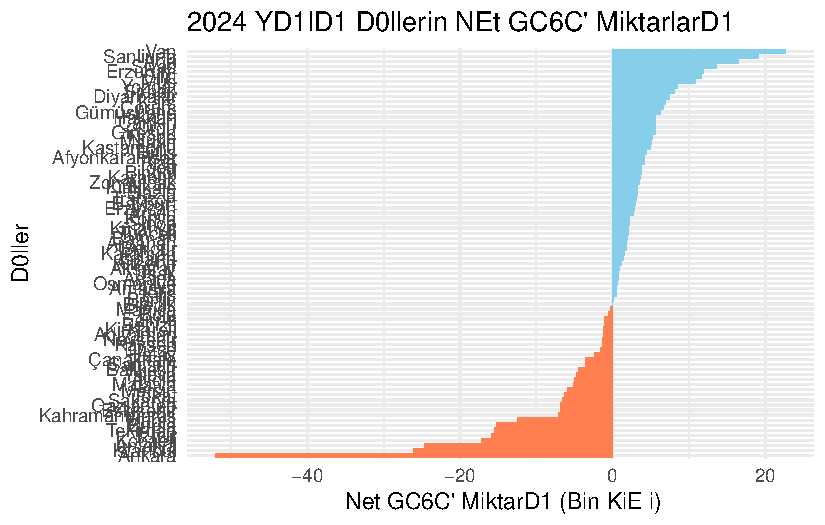
\includegraphics[keepaspectratio]{project_files/figure-pdf/unnamed-chunk-7-1.pdf}}

\subsubsection{3.1.5. Graph showing the distribution of migration
reasons that make up net migration
data.}\label{graph-showing-the-distribution-of-migration-reasons-that-make-up-net-migration-data.}

Migration reasons include: change of job, starting/finding a job, change
of marital status/family-related reasons, better housing and living
conditions, migration related to any member of the household/family,
returning to family home/hometown, health/care, buying a house,
retirement, other, and unknown.

\begin{Shaded}
\begin{Highlighting}[]
\NormalTok{NetGoc  }\OtherTok{\textless{}{-}} \FunctionTok{read\_excel}\NormalTok{(}\StringTok{"C:/Users/Public/Documents/my\_repository\_emu660/emu660{-}spring2026{-}burcubaris/NetGoc.xlsx"}\NormalTok{,}\AttributeTok{col\_names =} \ConstantTok{TRUE}\NormalTok{)}

\NormalTok{goc\_nedenleri }\OtherTok{\textless{}{-}} \FunctionTok{c}\NormalTok{(}\StringTok{"Tayin/Is Degisikligi"}\NormalTok{, }\StringTok{"Ise Baslamak/Is Bulmak"}\NormalTok{, }\StringTok{"Egitim"}\NormalTok{, }
                   \StringTok{"Medeni Durum/Ailevi"}\NormalTok{, }\StringTok{"Daha Iyi Konut/Yasam"}\NormalTok{, }\StringTok{"Haneye Bagimli Goc"}\NormalTok{, }
                   \StringTok{"Memlekete Donus"}\NormalTok{, }\StringTok{"Saglik/Bakim"}\NormalTok{, }\StringTok{"Ev Alinmasi"}\NormalTok{, }
                   \StringTok{"Emeklilik"}\NormalTok{, }\StringTok{"Diger"}\NormalTok{, }\StringTok{"Bilinmeyen"}\NormalTok{)}

\FunctionTok{colnames}\NormalTok{(NetGoc)[}\DecValTok{1}\SpecialCharTok{:}\DecValTok{3}\NormalTok{] }\OtherTok{\textless{}{-}} \FunctionTok{c}\NormalTok{(}\StringTok{"Yil"}\NormalTok{, }\StringTok{"Il"}\NormalTok{, }\StringTok{"Toplam\_Goc"}\NormalTok{)}
\FunctionTok{colnames}\NormalTok{(NetGoc)[}\DecValTok{4}\SpecialCharTok{:}\DecValTok{15}\NormalTok{] }\OtherTok{\textless{}{-}}\NormalTok{ goc\_nedenleri}
\NormalTok{veri\_2024 }\OtherTok{\textless{}{-}} \FunctionTok{subset}\NormalTok{(NetGoc, Yil }\SpecialCharTok{==} \DecValTok{2024} \SpecialCharTok{\&}\NormalTok{ Il }\SpecialCharTok{!=} \StringTok{"Toplam{-}Total"}\NormalTok{)}

\NormalTok{veri\_uzun }\OtherTok{\textless{}{-}} \FunctionTok{pivot\_longer}\NormalTok{(veri\_2024, }
                          \AttributeTok{cols =} \DecValTok{4}\SpecialCharTok{:}\DecValTok{15}\NormalTok{, }
                          \AttributeTok{names\_to =} \StringTok{"Goc\_Nedeni"}\NormalTok{, }
                          \AttributeTok{values\_to =} \StringTok{"Miktar"}\NormalTok{)}

\NormalTok{veri\_uzun}\SpecialCharTok{$}\NormalTok{Miktar\_Bin }\OtherTok{\textless{}{-}}\NormalTok{ veri\_uzun}\SpecialCharTok{$}\NormalTok{Miktar }\SpecialCharTok{/} \DecValTok{1000}

\NormalTok{goc\_grafigi }\OtherTok{\textless{}{-}} \FunctionTok{ggplot}\NormalTok{(veri\_uzun, }\FunctionTok{aes}\NormalTok{(}\AttributeTok{x =}\NormalTok{ Miktar\_Bin, }\AttributeTok{y =} \FunctionTok{reorder}\NormalTok{(Il, Toplam\_Goc), }\AttributeTok{fill =}\NormalTok{ Goc\_Nedeni)) }\SpecialCharTok{+}
  \FunctionTok{geom\_col}\NormalTok{(}\AttributeTok{position =} \StringTok{"stack"}\NormalTok{) }\SpecialCharTok{+}
  \FunctionTok{theme\_minimal}\NormalTok{() }\SpecialCharTok{+}
  \FunctionTok{labs}\NormalTok{(}
    \AttributeTok{title =} \StringTok{"2024 YD1lD1 D0llerin GC6C\textquotesingle{} Nedenlerine GC6re DaDD1lD1mD1"}\NormalTok{,}
    \AttributeTok{subtitle =} \StringTok{"Miktarlar bin kiEi cinsinden ifade edilmiEtir"}\NormalTok{,}
    \AttributeTok{x =} \StringTok{"Net GC6C\textquotesingle{} MiktarD1 (Bin KiEi)"}\NormalTok{,}
    \AttributeTok{y =} \StringTok{"D0ller"}\NormalTok{,}
    \AttributeTok{fill =} \StringTok{"GC6C\textquotesingle{} Nedenleri"}
\NormalTok{  ) }\SpecialCharTok{+}
  \FunctionTok{theme}\NormalTok{(}
    \AttributeTok{legend.position =} \StringTok{"bottom"}\NormalTok{,}
    \AttributeTok{legend.text =} \FunctionTok{element\_text}\NormalTok{(}\AttributeTok{size =} \DecValTok{8}\NormalTok{),}
    \AttributeTok{axis.text.y =} \FunctionTok{element\_text}\NormalTok{(}\AttributeTok{size =} \DecValTok{7}\NormalTok{)}
\NormalTok{  ) }\SpecialCharTok{+}
  \FunctionTok{guides}\NormalTok{(}\AttributeTok{fill =} \FunctionTok{guide\_legend}\NormalTok{(}\AttributeTok{ncol =} \DecValTok{3}\NormalTok{))}
  
\FunctionTok{print}\NormalTok{(goc\_grafigi)}
\end{Highlighting}
\end{Shaded}

\pandocbounded{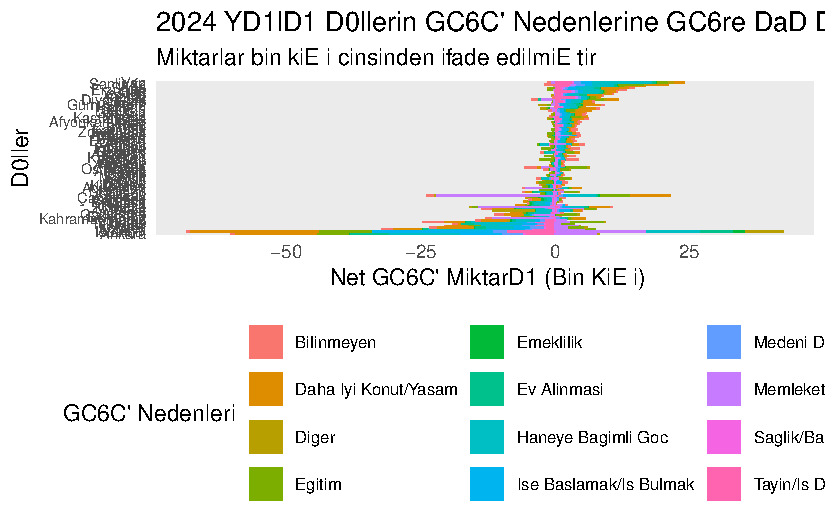
\includegraphics[keepaspectratio]{project_files/figure-pdf/unnamed-chunk-8-1.pdf}}

\subsection{3.2 Trend Analysis}\label{trend-analysis}

The graph shows the relational analysis between migration rate data and
life indices of the provinces.

```\{r\} yasam\_df \textless-
read\_excel(``C:/Users/Public/Documents/my\_repository\_emu660/emu660-spring2026-burcubaris/YasamEndeksi.xlsx'',
col\_names = TRUE) goc\_df \textless-
read\_excel(``C:/Users/Public/Documents/my\_repository\_emu660/emu660-spring2026-burcubaris/Gochizi.xlsx'',
col\_names = TRUE)

colnames(yasam\_df){[}1:2{]} \textless- c(``Il'', ``Endeks'')
colnames(goc\_df){[}1:3{]} \textless- c(``Yil'', ``Il'', ``Goc'')

goc\_2024 \textless- subset(goc\_df, Yil == 2024 \& Il !=
``Toplam-Total'')

veri\_seti \textless- inner\_join(yasam\_df, goc\_2024, by = ``Il'')

grafik \textless- ggplot(veri\_seti, aes(x = Endeks, y = Goc, label =
Il)) + geom\_point(color = ``\#1f77b4'', size = 3, alpha = 0.7) +
geom\_text\_repel(size = 3, max.overlaps = 15) + geom\_smooth(method =
``lm'', color = ``red'', se = TRUE, formula = y \textasciitilde{} x) +
labs( title = ``D0l YaEam Endeksi ve 2024 Net GC6C' HD1zD1 D0liEkisi'',
x = ``Genel Yasam Endeksi'', y = ``Net Goc Hizi (b




\end{document}
